
\section{The Dynamic Vision Sensor (DVS)\label{sec:The-DVS-camera}}

A regular CMOS camera records a visual scene by taking a stroboscopic
series of still frames. Computer vision and robot perception methods
work on the analysis of each frame separately. This established approach
has some fundamental drawbacks: each pixel gets sampled and processed
over and over again at each frame, independently of its relevance
to the decision to be taken, or whether its value changed. Much processing
power is used for considering redundant information, which translate
into high latencies and low frame rates. In contrast to this, we observe
that in biological systems there is redundancy suppression already
on the \textquotedblleft{}sensor\textquotedblright{}: as recordings
of nerve cells coming from the eye show, the retina mostly responds
to \emph{changes} in the perceived brightness.

The field of\emph{ neuromorphic engineering} tries to reproduce the
main characteristics of the computations done by nervous systems as
VLSI circuits. The computation is \emph{analogic}: currents, voltages
and charges are used for computing, rather than binary representations.
The resulting circuits are also \emph{asynchronous}: like nervous
cells, they operate independently of an external clock for state transitions.
There has been a large amount of research in neuromorphic sensory
systems of different scale and complexity~\cite{liu10neuromorphic}.
The first system to be commercially available is the so-called ``silicon
retina'' or Dynamic Vision Sensor\emph{ }(DVS)~\cite{lichtsteiner08asynchronous}.

Each pixel in the DVS operates independently and asynchronously from
the others. The photons that reach a photodiod produce a photocurrent,
which is converted into a voltage. This voltage gets continuously
compared to the last sampled voltage. As soon as the difference between
these two voltages is larger than a certain threshold, the pixel requests
to send an \emph{event} off chip. After the address and the timestamp
of this event has been registered from a CPLD at the chip periphery,
the pixel is reset, and the most recent voltage gets sampled to be
compared against successive voltages. All of this computation is done
without digitizing the signal. 

Each event carriers the following information: a timestamp, which
has a 1~\textmu{}s resolution, the \emph{address }of the pixel that
observed the change (equivalent to its~$x,y$ coordinates), and the
\emph{polarity} of the change (\pP or \pN). The polarity depends
on the sign of the difference. \pP~events indicate that the brightness
increased, while \pN~events indicated that it decreased.

The parameters that modulate the pixel behavior are dynamically programmed
using a set of bias currents. Some of the parameters that can be dynamically
changed are the temporal contrast frequency cutoff, the \pP \& \pN
threshold, and the event frequency cutoff. 

The sensor therefore only produces output if the observed scene changes.
This is not only the case if the intensity of a light source gets
modulated (as with a blinking LED), but also if a static scene moves
relative to the sensor. If the sensor itself is moved it perceives
all the edges and contours in its visual field.

Sensing the world with a set of autonomous, change-sensitive pixels
has various advantages compared to traditional image sensors:
\begin{itemize}
\item Since the photocurrent gets converted to a voltage on pixel level,
the brightness measurement does not require a uniform exposure time
for all pixels. This leads to the high dynamic range of 120dB which
is capped by the exposure time in conventional image sensors.
\item By only sensing changes, the sensor performs on-chip data compression.
This does not only make the amount of output data dependent on the
activity in a scene, but it also focuses the processing effort on
the region of interest where it is changing. This focusing allows
to create controllers that have update intervals of down to 125~\textmu{}s~\cite{conradt09pencil}.
\item Redundant information does not occupy the output bus and therefore
relevant information can be signaled very fast. The sensor chip itself
has a latency of 15~\textmu{}s. In practice the main limitation to
the latency of prototype systems is not the DVS, but USB communication.
Round-trip latencies of the whole systems using off-the-shelf computer
architectures are in the order of 3~ms~\cite{delbruck07fast}.
\item The high resolution of the event timestamps can be used to investigate
highly dynamics elements in a scene, such as fast motion or, like
in this paper, blinking LEDs. Moreover, because events are asynchronous,
it is not necessary to commit to use a given sampling frequency like
in a conventional sensors.
\end{itemize}
\begin{figure}[b]
\centering{}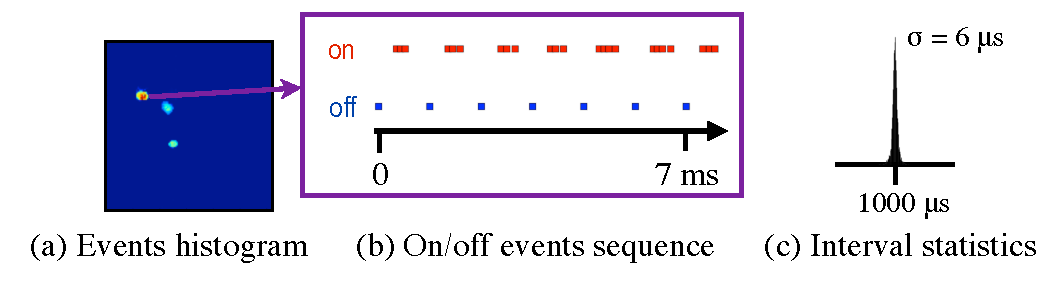
\includegraphics[bb=12bp 0bp 500bp 135bp,clip,width=8.6cm]{figures/slides/event_sequence2}\caption{\label{fig:events-hist}Example event sequence from a DVS looking
at an Active LED Marker (\ALM). Subfigure (a) shows the histogram
of events seen from a fixed camera looking at three \ALMs. The difference
in numbers is due to the different frequencies of the \ALMs. Subfigure
(b) shows a slice of the events seen at a particular pixel near the
center of one of the \ALMs which has a blinking frequency of 1 KHz.
The data is a series of events with positive (\pP) and negative (\pN)
events. (c) The sequence of \pPN transitions are highly regular;
in this data we observed that the distribution of the intervals is
well approximated by a Gaussian with mean $1000\,\mu s$ and standard
deviation $\sigma=6\,\mu s$. }
\end{figure}


The main drawbacks of the current generation of DVS are its low resolution
of $128\times128$, and the inability to sample the absolute brightness
levels like a normal camera. The low resolution is due to the prototype
fabrication process used (350~nm) and the fact that each pixel is
associated to a complex circuit carrying on the analog computation.
The absolute brightness levels cannot be accessed because the according
technology was not ready for the first series of sensors. But since
the field of event-based vision sensors is steadily growing~\cite{delbruck10activity},
these limitations will soon be overcome. Some of the latest developments
include higher temporal contrast sensitivity of 1.5\%~\cite{serrano13128}
and higher spatial resolution of~$240\times180$ or~$304\times240$,
accompanied with a readout channel for pictures and movies that simulates
a CMOS camera~\cite{posch11qvga,berner13240}. 

Other ongoing efforts include increasing the availability of the embedded
version of the sensor (eDVS, used in~\cite{conradt09pencil}), which
weighs only a few grams and measures~$30\times50\times50$~mm. Furthermore,
future versions of event based vision sensors are expected to include
a USB 3.0 interface for higher data transmission rates.
